\chapter{진동자 파동함수, 스핀 1/2, 입자 교환}

\section{곳곳에 있는 진동자}

안정한 평형 상태에 있는 계는 그 평형 상태에서 벗어나면 진동할 수 있다. 진동수는 하나일 수도 있고 여러 개일 수도 있다. 예를 들어 바이올린 현에는 기본 모드와 고조파가 있다. 현을 뜯으면 이 모드들이 어떤 조합으로 여기된다.

여기서 더 중요한 예는 장이다. 전자기장의 평형 배치는 진공이다. 즉, 전기장도 자기장도 전자기적 진동도 없다. 복사를 공동이나 도파관에 넣으면 장은 허용된 모드로 진동할 수 있으며, 각 모드는 고유한 진동수를 가진다. 양자 이론에서 이 모드들은 광자들의 집합을 나타낸다.

같은 생각은 결정에도 적용된다. 모든 원자를 서로 독립된 진동자로 보는 것은 오해를 부른다. 원자들은 서로 힘을 주고받으므로 한 원자의 변위는 이웃 원자에 영향을 미치고, 파동은 결정을 따라 전파된다. 이렇게 결합된 운동의 정상 모드는 조화 진동자이며, 그 양자를 포논이라고 한다. 광자와 포논은 서로 다른 물리적 대상이지만, 둘 다 같은 진동자 대수로 이어진다.

\section{진동자 대수}

진동자를 논의하는 동안 질량과 환산 플랑크 상수를 1로 둔다:
\[
m=1,\qquad \hbar=1.
\]
해밀토니안은 다음과 같다.
\begin{equation}
H=\frac{p^{2}}{2}+\frac{\omega^{2}x^{2}}{2}.
\end{equation}
매개변수 \(\omega\)는 퍼텐셜의 곡률을 정하며, 진동수이기도 하다.

상승 연산자와 하강 연산자를 다음과 같이 정의한다.
\begin{equation}
A_{\pm}=\frac{p\pm i\omega x}{\sqrt{2\omega}}.
\end{equation}
정규화는 다음 관계가 성립하도록 정한다.
\begin{equation}
[A_{-},A_{+}]=1.
\end{equation}
수 연산자는 다음과 같다.
\begin{equation}
N=A_{+}A_{-}.
\end{equation}
이 식들로부터 \(A_{+}\)는 \(N\)의 고유값을 1만큼 높이고, \(A_{-}\)는 1만큼 낮춘다는 것을 알 수 있다. 따라서 스펙트럼은 다음과 같다.
\begin{equation}
n=0,1,2,3,\ldots .
\end{equation}

두 사다리 연산자를 곱하면 고전적 에너지에 대한 양자 보정도 드러난다.
\begin{align}
N
&=\frac{1}{2\omega}(p+i\omega x)(p-i\omega x)\\
&=\frac{1}{2\omega}\left(p^{2}+\omega^{2}x^{2}
 +i\omega[x,p]\right)\\
&=\frac{1}{2\omega}\left(p^{2}+\omega^{2}x^{2}-\omega\right),
\end{align}
여기서 \([x,p]=i\)이다. 따라서
\begin{equation}
H=\omega\left(N+\frac12\right).
\end{equation}
가산 상수가 문제와 무관하다면, 다음과 같이 평행이동한 해밀토니안을 쓰는 것이 편리하다.
\begin{equation}
H_{\mathrm{shifted}}=H-\frac{\omega}{2}=\omega N.
\end{equation}
항 \(\omega/2\)는 진동자의 영점 에너지, 즉 바닥 상태 에너지다. 장 모드에서 이에 해당하는 항은 진공 에너지라고 한다. 이는 불확정성 원리를 반영한다. 어떤 상태에서도 \(x\)와 \(p\)가 모두 정확히 0일 수 없으므로, \(H\)의 두 양의 이차항이 모두 기댓값 0을 가질 수는 없다.

\begin{classroomqa}
\lecturetimestamp{00:09:46}
\audiencequestion{수 연산자의 스펙트럼에 0이 포함되는 이유는 무엇인가요?}
\lecturerresponse{바닥 상태 파동함수를 구성하면 이를 명시적으로 보일 수 있습니다. 그 구성으로 \(N=0\)인 상태를 확인하겠습니다.}
\end{classroomqa}

이 구성을 시작하기 위해 상태 벡터를 위치의 파동함수로 바꿔 표현하자. 에너지 고유상태는 다음과 같이 된다.
\[
\psi_{0}(x),\ \psi_{1}(x),\ \psi_{2}(x),\ldots,
\]
기본 연산자들은 다음과 같이 작용한다.
\begin{equation}
X\longmapsto x,\qquad
P\longmapsto -i\frac{d}{dx}.
\end{equation}
\(\hbar\)를 다시 넣으면 두 번째 대응은 다음과 같다.
\(P\mapsto-i\hbar\,d/dx\).

\(\psi_{0}\)를 구하기에 앞서 질문에 대한 더 빠른 추상적 답이 있다. 정규화 가능한 진동자 고유상태의 이산 사다리에서 \(N=A_{+}A_{-}\)는 음이 아닌 값이므로, 단위 간격으로 계속 낮추는 일을 무한히 이어갈 수는 없다. 그 끝점---아래에서 정규화 가능한 파동함수를 구성할 것이다---에는 다음을 만족하는 상태가 있어야 한다. 이 상태를 \(\lvert0\rangle\)라 쓰자.
\begin{equation}
A_{-}\lvert0\rangle=\mathbf 0.
\end{equation}
그렇지 않다면 \(A_{-}\lvert0\rangle\)는 한 단계 더 낮은 또 다른 상태일 것이다. 따라서 곧바로 다음을 얻는다.
\begin{equation}
N\lvert0\rangle
=A_{+}A_{-}\lvert0\rangle
=\mathbf 0
=0\,\lvert0\rangle.
\end{equation}
그러므로 가장 낮은 상태의 수 고유값은 0이다.

\begin{classroomqa}
\lecturetimestamp{00:14:57}
\audiencequestion{고유값이 0이라면 우변에 영 고유벡터가 있어야 하지 않나요?}
\lecturerresponse{켓 \(\lvert0\rangle\)는 정규화된 0이 아닌 벡터이며, 그 표지가 0이다. \(N\lvert0\rangle=0\,\lvert0\rangle\)에서 우변은 영벡터다. 바닥 상태 켓과 영벡터는 서로 다른 대상이다.}
\end{classroomqa}

\section{Schr\"odinger 방정식과 물리적 해}

이제 위치 표현으로 돌아가자. 시간에 무관한 Schr\"odinger 방정식은 다음과 같다.
\begin{equation}
\left[
-\frac12\frac{d^{2}}{dx^{2}}
+\frac12\omega^{2}x^{2}
\right]\psi(x)=E\psi(x).
\end{equation}
이 방정식은 2계 미분방정식이므로 \(E\)의 임의의 값에 대한 형식적 해를 가진다. 하지만 이 형식적 해의 대부분은 물리적인 진동자 상태가 아니다. 이 해들은 큰 \(\lvert x\rvert\)에서 지수적으로 증가하여 노름이 발산한다.

속박 상태의 파동함수는 제곱 적분 가능해야 한다.
\begin{equation}
\int_{-\infty}^{\infty}\psi^{*}(x)\psi(x)\,dx<\infty.
\end{equation}
그러면 적분값이 1이 되도록 정규화할 수 있다. 특별한 에너지 값에서만 이런 해가 나온다. 무한 직선 위의 위치 상태와 운동량 상태는 이 점에서 예외지만, 지수적으로 증가하는 진동자 해는 상태 공간에서 제외된다.

\section{가우스 바닥 상태}

2계 방정식을 풀 수도 있지만, 사다리 대수를 이용하면 더 간단한 1계 방정식을 얻는다.
\begin{equation}
A_{-}\psi_{0}(x)=0.
\end{equation}
우변이 0이므로 \(A_{-}\) 앞의 전체 인자는 중요하지 않다. 따라서 다음과 동등하다.
\begin{equation}
(p-i\omega x)\psi_{0}(x)=0.
\end{equation}
\(p=-i\,d/dx\)를 사용하면 다음과 같다.
\begin{equation}
\left(\frac{d}{dx}+\omega x\right)\psi_{0}(x)=0.
\end{equation}

\begin{classroomqa}
\lecturetimestamp{00:22:32}
\audiencequestion{변수분리법으로 풀 수 있나요?}
\lecturerresponse{독립변수가 하나뿐이므로 분리할 두 변수가 없다. \(\psi_{0}'/\psi_{0}=-\omega x\)처럼 쓰면 이 방정식은 로그 미분의 형태다. 따라서 파동함수를 지수함수로 놓는 것이 자연스럽다.}
\end{classroomqa}

이를 푸는 유용한 방법은 다음과 같이 놓는 것이다.
\begin{equation}
\psi_{0}(x)=e^{f(x)}.
\end{equation}
그러면
\[
\psi_{0}'(x)=f'(x)e^{f(x)},
\]
공통 지수 인자는 약분된다. 방정식은 다음과 같이 간단해진다.
\begin{equation}
\frac{df}{dx}+\omega x=0.
\end{equation}

\begin{classroomqa}
\lecturetimestamp{00:26:28}
\audiencequestion{\(f(x)\)에 마이너스 부호가 있어야 하지 않나요?}
\lecturerresponse{그렇다. \(df/dx=-\omega x\)이므로 적분하면 음의 이차항이 나온다.}
\end{classroomqa}

따라서
\begin{equation}
f(x)=-\frac12\omega x^{2}+C,
\end{equation}
그리고
\begin{equation}
\psi_{0}(x)\propto e^{-\omega x^{2}/2}.
\end{equation}
곱셈 정규화 상수는 정하지 않은 채 둔다. 중요한 점은 가우스 형태라는 것이다. 이 파동함수는 매끄럽고 원점 부근에 집중되어 있으며, 큰 \(\lvert x\rvert\)에서 빠르게 감소한다. 명백히 제곱 적분 가능하다.

에너지를 알아내기 위해 답을 2계 방정식에 다시 대입할 필요는 없다. 대수에서 이미 다음을 얻었다.
\begin{equation}
E_{0}=\frac{\omega}{2}.
\end{equation}

\section{들뜬 상태, 마디, 고전적 운동}

첫 번째 들뜬 상태는 바닥 상태에 상승 연산자를 작용시켜 얻는다.
\begin{equation}
\psi_{1}(x)\propto A_{+}\psi_{0}(x)
\propto(p+i\omega x)e^{-\omega x^{2}/2}.
\end{equation}
바닥 상태 방정식은 다음과 같다.
\[
p\psi_{0}=i\omega x\,\psi_{0}.
\]
사다리 연산자의 부호를 바꾸면 상쇄가 덧셈으로 바뀐다.
\begin{equation}
(p+i\omega x)\psi_{0}
=2i\omega x\,\psi_{0}.
\end{equation}
전체 상수 인자를 제외하면
\begin{equation}
\psi_{1}(x)\propto x\,e^{-\omega x^{2}/2}.
\end{equation}

이 파동함수는 홀함수다.
\begin{equation}
\psi_{1}(-x)=-\psi_{1}(x).
\end{equation}
확률밀도는 짝함수지만 원점에 마디가 있다.
\begin{equation}
\lvert\psi_{1}(0)\rvert^{2}=0.
\end{equation}
따라서 첫 번째 들뜬 상태의 확률밀도에는 \(x=0\)에 마디가 있다.

\(A_{+}\)를 반복해서 작용시키면 같은 가우스 포락선에 더 높은 차수의 다항식이 곱해진 형태가 나온다.\footnote{\(00{:}34{:}25\)에서 \(00{:}35{:}49\)까지 강의에서는 더 높은 차수의 다항식 인자와 매 단계 추가되는 마디, 그리고 번갈아 나타나는 대칭성을 설명한다. 가우스 함수와 다항식의 곱이라는 형태는 Leonard Susskind와 Art Friedman의 \emph{양자역학: 이론적 최소}(2014)에서 진동자 고유함수를 다루는 부분에서도 확인할 수 있다.}정규화 상수를 제외하면
\begin{equation}
\psi_{n}(x)=P_{n}(x)e^{-\omega x^{2}/2}.
\end{equation}
짝홀성은 짝함수와 홀함수 사이에서 번갈아 나타나고, 단계마다 마디가 하나씩 추가된다. \(n\)가 커질수록 파동함수는 원점에서 더 멀리 퍼지고 더 빠르게 진동한다.

이 두 특징은 물리적 의미가 분명하다. 퍼텐셜이 \(x^{2}\)에 비례해 커지므로 원점에서 더 멀리까지 퍼지는 것은 더 큰 퍼텐셜 에너지에 해당한다. 위치 공간에서 빠른 진동은 더 큰 운동량을 나타낸다. 크게 들뜬 진동자는 중심에서 더 멀리까지 나아갈 가능성이 크다. 중심 영역을 지날 때에는 운동량이 더 크고 파동함수도 그곳에서 더 빠르게 진동한다.

\begin{classroomqa}
\lecturetimestamp{00:37:18}
\audiencequestion{\(n\)가 커져도 조화 진동자는 고전적 거동에 가까워지지 않나요?}
\lecturerresponse{고전적 운동은 하나의 정상 에너지 고유상태로 표현되지 않는다. 여러 에너지 준위를 포함하는 파동 묶음으로 나타난다. 예를 들어 변위된 가우스 파동 묶음은 고전적 진동자처럼 앞뒤로 움직이며, 진폭이 커질수록 상대적 불확정성이 작아진다.}
\end{classroomqa}

바닥 상태 가우스 파동함수에서 시작해 원점으로부터 변위시키자. 변위된 파동 묶음은 더 이상 에너지 고유상태가 아니라 여러 고유상태의 중첩이다. 시간에 따른 Schr\"odinger 방정식에 따라 각 성분은 서로 다른 위상을 얻는다. 파동 묶음은 퍼텐셜의 한쪽에서 다른 쪽으로 진동하며, 중심 부근에서는 위상이 빠르게 변하고 전환점 부근에서는 다시 매끄러워진다. 파동 묶음의 폭에 비해 진폭이 클수록 운동은 고전적인 것에 더 가까워 보인다.

\begin{classroomqa}
\lecturetimestamp{00:39:29}
\audiencequestion{두 번째 들뜬 상태의 파동함수는 원점에서 영점을 지나야 하나요?}
\lecturerresponse{아닙니다. 다항식 인자는 단순히 \(x^{2}\)만이 아니라 상수항도 포함하므로, 파동함수가 \(x=0\)에서 반드시 0이 될 필요는 없습니다.}
\end{classroomqa}

사다리 논증은 또한 제곱 적분 가능한 진동자 정의역에서 \(A_{+}\)와 \(A_{-}\)가 에르미트 켤레이며, 수반 관계에 필요한 경계 거동을 만족한다고 가정한다. 지수적으로 증가하는 형식적 해는 이 정의역에 속하지 않는다.

\begin{classroomqa}
\lecturetimestamp{00:40:45}
\audiencequestion{해밀토니안이 이런 대수적 방법으로 풀릴 수 있는지 알아보는 일반적인 방법이 있나요?}
\lecturerresponse{그런 종류의 일반적인 규칙은 없다. 정확히 풀 수 있는 예는 드물다. 조화 진동자와 이상적인 비상대론적 수소 원자는 대수적 방법이 통하는 운 좋은 사례다.}
\end{classroomqa}

\section{각운동량으로서의 스핀 1/2}

스핀은 입자의 질량중심 궤도 운동과 별개로 입자가 지닌 각운동량이다. 정지한 입자에는 궤도 각운동량 \(\mathbf R\times\mathbf P\)가 없지만, 스핀은 여전히 있을 수 있다. 아주 작은 회전 물체를 떠올릴 수도 있고, 스핀을 고유한 양자 성질로 다룰 수도 있다. 핵심은 수학적 진술에 있다. 스핀의 성분은 공간 회전 아래에서 변환하며 각운동량 교환 관계를 따른다.

이제부터 \(\hbar\)를 다시 넣는다. 각운동량 성분은 다음 관계를 만족한다.
\begin{equation}
[L_{z},L_{x}]=i\hbar L_{y},
\end{equation}
나머지 두 관계는 첨자를 순환 치환하여 얻는다. 무차원 파울리 행렬은 다음과 같다.
\begin{equation}
\begin{aligned}
\sigma_{z}&=
\begin{pmatrix}
1&0\\
0&-1
\end{pmatrix},\\[0.4em]
\sigma_{x}&=
\begin{pmatrix}
0&1\\
1&0
\end{pmatrix},\\[0.4em]
\sigma_{y}&=
\begin{pmatrix}
0&-i\\
i&0
\end{pmatrix}.
\end{aligned}
\end{equation}
이 기저에서 \(\sigma_{z}\)는 대각 행렬이다. 고유값은 \(+1\)와
\(-1\)이다.

\begin{classroomqa}
\lecturetimestamp{00:47:35}
\audiencequestion{\(\sigma_x\)에는 마이너스 부호가 있나요?}
\lecturerresponse{아니다. \(\sigma_x\)의 두 비대각 성분은 모두 양수다.}
\end{classroomqa}

\(00{:}49{:}35\)의 판서 계산은 각 성분의 곱을 구하기 시작한다. 곱셈을 마치면 다음과 같다.
\begin{align}
\sigma_{z}\sigma_{x}
&=
\begin{pmatrix}
0&1\\
-1&0
\end{pmatrix}
=i\sigma_{y},\\
\sigma_{x}\sigma_{z}
&=
\begin{pmatrix}
0&-1\\
1&0
\end{pmatrix}
=-i\sigma_{y}.
\end{align}
따라서
\begin{equation}
[\sigma_{z},\sigma_{x}]=2i\sigma_{y}.
\end{equation}
물리적 스핀 연산자를 다음과 같이 정의하면 추가된 2라는 인자가 사라진다.\footnote{\(\hbar\)는 판서 계산에서 생략했다. \(S_i\)가 각운동량의 단위를 갖도록 여기서는 이를 다시 넣었다.}
\begin{equation}
S_{i}=\frac{\hbar}{2}\sigma_{i}.
\end{equation}
그러면
\begin{equation}
[S_{z},S_{x}]=i\hbar S_{y},
\end{equation}
첨자를 순환 치환한 경우도 마찬가지다. 따라서 복원된 \(\hbar\) 인자를 포함한 파울리 행렬의 절반은 각운동량 계를 이룬다.

\(\hbar=1\)로 두면 아래와 같은 형태가 된다.\footnote{원본 자료의 프레임은 \texttt{강의\_04\_프레임\_02.png}이다.}
\begin{figure}[htbp]
\centering
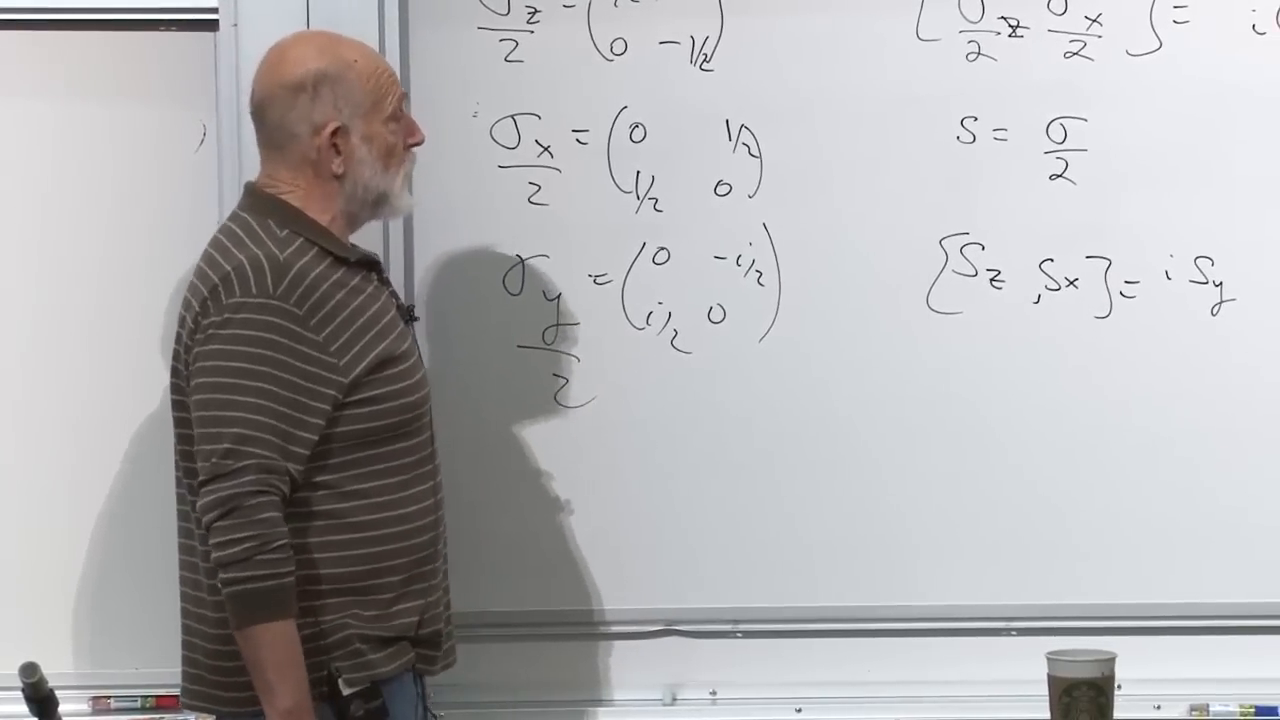
\includegraphics[width=0.9\linewidth]{lecture_04_frame_02.png}
\caption{\(\hbar=1\)인 단위계에서 파울리 행렬의 절반은 스핀 1/2 각운동량 연산자이며 \([S_z,S_x]=iS_y\)을 만족한다.}
\lectureframe{00:55:41}
\end{figure}

두 \(S_z\) 고유값 방정식은 다음과 같다.
\begin{equation}
S_z\lvert\pm\rangle
=\pm\frac{\hbar}{2}\lvert\pm\rangle.
\end{equation}
동등하게, 무차원 자기 양자수는 다음과 같다.
\begin{equation}
m_{s}=\pm\frac12,
\qquad
S_{z}\lvert m_{s}\rangle
=m_{s}\hbar\,\lvert m_{s}\rangle.
\end{equation}
각운동량 상승 연산자와 하강 연산자는 \(m\)를 정수 간격으로 바꾸지만, 그렇다고 모든 사다리가 0을 거쳐야 하는 것은 아니다. 정수 다중항은 정수 \(m\)값을 포함하고, 반정수 다중항은 반정수 값을 포함한다. 스핀 1/2의 사다리에는 \(m_s=+1/2\)와 \(m_s=-1/2\)라는 두 상태만 있다.

이 두 상태는 스핀 1/2 이중항을 이룬다. 전자, 뮤온, 중성미자, 쿼크는 이런 반정수 스핀 다중항으로 기술되는 입자에 속한다.

\section{궤도 각운동량과 스핀 각운동량}

이제 두 종류의 각운동량이 있다. 궤도 각운동량은 원점에 대한 운동을 나타내며,
\begin{equation}
\mathbf L=\mathbf R\times\mathbf P,
\end{equation}
\(\mathbf S\)는 고유한 스핀이다. 이 둘의 벡터 합은 전체 각운동량이다.
\begin{equation}
\mathbf J=\mathbf L+\mathbf S.
\end{equation}

\begin{classroomqa}
\lecturetimestamp{00:56:49}
\audiencequestion{계의 전체 각운동량이 \(\mathbf J\)라면 스핀 \(\mathbf S\)은 어떻게 알아내나요?}
\lecturerresponse{스핀 양자수와 궤도 양자수는 보통 별도로 주어진다. \(L=0\)라면 각운동량은 모두 스핀이다. 그렇지 않으면 각운동량을 더하는 양자 규칙이 필요하지만, 여기서는 뒤로 미룬다.}
\end{classroomqa}

각운동량 덧셈 규칙은 궤도 각운동량과 스핀을 더하는 경우, 두 스핀을 더하는 경우, 두 궤도 각운동량을 더하는 경우에 똑같이 적용된다. 결합된 계는 허용되는 자체의 전체 각운동량 값을 가지지만, 아직 그 규칙을 쓸 필요는 없다.

\begin{classroomqa}
\lecturetimestamp{00:58:18}
\audiencequestion{스핀을 도입하게 된 실험적 증거는 무엇이었나요?}
\lecturerresponse{분광학이 증거를 제공했지만, 주기율표는 특히 명료한 동기를 보여준다. 주기율표의 껍질 구조를 설명하려면 전자에 두 값을 갖는 추가 성질이 있어야 한다.}
\end{classroomqa}

\section{수소형 원자의 축퇴와 껍질 상태 수 세기}

궤도 각운동량의 경우 \(L^{2}\) 고유값 방정식은 다음과 같다.
\begin{equation}
L^{2}\lvert\ell,m\rangle
=\hbar^{2}\ell(\ell+1)\lvert\ell,m\rangle,
\end{equation}
\(\ell\)의 고정된 값에 대해 자기 상태는
\begin{equation}
2\ell+1
\end{equation}
개이며, 이에 해당하는 값은 \(m=-\ell,-\ell+1,\ldots,\ell\)이다.

이상적인 비상대론적 쿨롱 문제에는 추가적인 축퇴가 있다. 속박 상태의 에너지는 음수이며 아래쪽에서 0에 가까워지지만, 상태 수를 셀 때는 준위가 어떻게 겹치는지만 중요하다. 첫 번째 \(\ell=1\) 준위는 다음 \(\ell=0\) 준위와 같은 에너지에 놓이고, 첫 번째 \(\ell=2\) 준위는 다음 주양자수 껍질의 준위와 겹친다. 이 패턴은 계속된다.\footnote{\texttt{\_강의04\_\_프레임03}, \(01{:}02{:}01\); 완성된 주양자수 껍질의 준위 정렬은 \(01{:}02{:}33\)부터 \(01{:}04{:}10\)까지 설명된다.}

\begin{figure}[htbp]
\centering
\begin{tikzpicture}[x=1.55cm,y=1.0cm]
\draw[->] (-0.65,0) -- (-0.65,4.35);
\draw[->] (-0.85,0) -- (4.75,0);
\node at (-0.95,4.08) {\(E\)};
\node at (4.55,-0.28) {\(\ell\)};
\node at (0,-0.30) {\(0\)};
\node at (2,-0.30) {\(1\)};
\node at (4,-0.30) {\(2\)};

\draw (-0.20,0.75) -- (0.20,0.75);

\draw (-0.20,2.00) -- (0.20,2.00);
\foreach \dx in {-0.18,0,0.18}
  \draw (2+\dx-0.06,2.00) -- (2+\dx+0.06,2.00);

\draw (-0.20,3.15) -- (0.20,3.15);
\foreach \dx in {-0.18,0,0.18}
  \draw (2+\dx-0.06,3.15) -- (2+\dx+0.06,3.15);
\foreach \dx in {-0.32,-0.16,0,0.16,0.32}
  \draw (4+\dx-0.05,3.15) -- (4+\dx+0.05,3.15);

\node[anchor=west] at (0.35,0.75) {\(n=1\)};
\node[anchor=west] at (2.35,2.00) {\(n=2\)};
\node[anchor=west] at (4.40,3.15) {\(n=3\)};
\end{tikzpicture}
\caption{이상적인 쿨롱 문제의 처음 세 껍질에는 같은 주양자수 에너지를 갖는 궤도 다중항들이 함께 들어간다. 첫 번째 껍질에는 한 상태, 두 번째에는 \(1+3\), 세 번째에는 \(1+3+5\)가 있다.}
\lectureframe{01:02:01}
\end{figure}

주양자수 껍질 \(n\)에서 허용되는 궤도 각운동량 값은\footnote{이 간결한 \(\ell\) 범위와 아래의 합으로 준위의 정렬과 \(1,4,9,16,\ldots\)의 개수를 재구성할 수 있으며, 이는 \(01{:}02{:}33\)부터 \(01{:}04{:}10\)까지 설명된다. 스펙트럼 그림의 시작 부분은 \texttt{강의\_04\_프레임\_03.png}의 \(01{:}02{:}01\)에서 볼 수 있다.}
\[
\ell=0,1,\ldots,n-1.
\]
따라서 공간 상태의 수는 다음과 같다.
\begin{equation}
\sum_{\ell=0}^{n-1}(2\ell+1)=n^{2},
\end{equation}
이에 따른 수열은 다음과 같다.
\begin{equation}
1,\ 4,\ 9,\ 16,\ldots .
\end{equation}
여기까지는 궤도 상태만 센 것이다. 각 공간 상태에는 두 스핀 값이 가능하므로, 이에 대응하는 이상화된 총수는 다음과 같다.
\begin{equation}
2,\ 8,\ 18,\ 32,\ldots=2n^{2}.
\end{equation}

\section{배타 원리와 전자의 두 값 성질}

먼저 독립 전자 근사에서 헬륨을 생각하자. 헬륨의 핵은 양성자 전하가 두 배이므로 수소형 에너지 준위의 척도가 바뀌고 전자들이 안쪽으로 끌려온다. 우선 전자--전자 상호작용을 무시하면, 전자 두 개가 가장 낮은 공간 궤도에 들어갈 수 있고 이는 헬륨 바닥 상태의 첫 근사로 꽤 타당하다.

그렇다면 왜 전자를 하나 더 넣지 않을까? 궤도 에너지는 더 낮아지겠지만, 실제로는 그런 일이 일어나지 않는다. 이를 제한하는 원리는 파울리 배타 원리다. 두 전자는 같은 완전한 1입자 상태를 차지할 수 없다. 이를 일반적인 반발력이라고 부르면 오해를 낳는다. 이는 허용되는 양자 상태에 대한 제약이다.

겉보기에는 모순이 있다. 헬륨의 전자 두 개는 실제로 같은 공간 궤도를 차지한다. 완전한 전자 상태에는 궤도 파동함수보다 더 많은 것이 들어 있다는 점이 이 모순을 풀어준다. 전자 상태에는 두 값을 갖는 자유도도 있다. 그 값을 위와 아래라고 하자. 가장 낮은 궤도에 있는 한 전자는 스핀 위, 다른 전자는 스핀 아래일 수 있다. 두 전자의 공간 상태는 같지만 전체 양자 상태는 다르다.

이제 상태 수 세기는 리튬을 향해 진행하다가 다시 되짚는다. 이 되짚기로 배타 원리와 스핀이 모두 필요한 이유가 드러난다. 스핀은 전혀 없고 배타 규칙만 있다고 상상해 보자. 가장 낮은 공간 상태에는 전자 하나만 들어갈 수 있다. 두 번째 전자는 다음 주양자수 껍질의 공간 상태 네 개 중 하나에 들어가야 한다. 그러면 관측된 헬륨 바닥 상태는 하나뿐인데도 여러 대안이 생긴다. 스핀이 없는 이런 배타 규칙은 틀렸다.

두 스핀 값을 다시 포함하자. 전자 두 개는 가장 낮은 궤도를 반대 스핀으로 채운다. 중성 리튬에서처럼 세 번째 전자는 다음 주양자수 껍질에 들어가야 한다. 그 껍질에는 \(\ell=0\) 공간 상태 하나와 \(\ell=1\) 공간 상태 세 개가 있다. 스핀을 세기 전에는 가능성이 네 가지다.

\begin{classroomqa}
\lecturetimestamp{01:14:58}
\audiencequestion{\(s\) 상태와 \(p\) 상태는 어떻게 해서 첫 번째 들뜬 껍질에서 여덟 가지 가능성을 만드나요?}
\lecturerresponse{공간 상태는 \(\ell=0\)인 것이 하나, \(\ell=1\)인 것이 세 개이므로 모두 네 개다. 각각에 두 스핀 값이 가능하므로 전체는 \(2(1+3)=8\)이다.}
\end{classroomqa}

이것이 주기율표 두 번째 행의 여덟 원소를 설명하는 간단한 상태 수 세기다. 이는 의도적으로 이상화한 설명이다. 뒤에서 보겠지만, 전자--전자 상호작용 때문에 독립적인 수소형 껍질 그림은 곧 무너진다.

두 값 성질이 각운동량인지도 시험할 수 있다. 전자 스핀에는 자기 모멘트가 따르므로, 자기장은 두 스핀 투영에 서로 다른 에너지를 부여한다. 영자기장에서 축퇴되어 있던 준위가 두 개로 갈라진다. 이는 작은 자기 모멘트가 장과 나란히 또는 반대로 정렬할 때 예상되는 것과 같다. 이 분리는 추가된 두 값 자유도가 임의의 이진 표지가 아니라 각운동량으로 거동하는지 시험한다.

\section{광자, 전자, 그리고 껍질 그림의 한계}

모든 입자가 같은 점유 규칙을 따르는 것은 아니다. 여러 광자가 같은 전자기 모드를 점유할 수 있다. 고전적인 빛의 파동은 그 모드에 많은 광자가 들어 있는 상태로 이해할 수 있다. 전자는 다르게 거동한다. 배타 원리는 전자들이 하나의 완전한 양자 상태에 몰려드는 것을 막는다. 이런 차이로 두 가지 입자 통계가 구분된다.

\begin{classroomqa}
\lecturetimestamp{01:20:28}
\audiencequestion{원자에 속박된 전자가 아니라 자유롭게 흐르는 전자 다발이라면 어떻게 되나요?}
\lecturerresponse{배타 규칙은 여전히 적용된다. 전자들이 모두 하나의 양자 상태를 차지할 수는 없다. 레이저는 많은 광자를 같은 모드에 넣을 수 있지만, 전자 다발은 그런 식으로 만들 수 없다.}
\end{classroomqa}

이 제약은 전자의 성질이지 원자에 속박되어 있다는 특이성 때문이 아니다.

\begin{classroomqa}
\lecturetimestamp{01:21:12}
\audiencequestion{궤도 각운동량은 특별히 핵 주위의 회전을 뜻하나요?}
\lecturerresponse{각운동량은 선택한 원점을 기준으로 정의한다. 원자는 핵을 자연스러운 원점으로 삼지만, 자유 입자의 각운동량은 어떤 원점을 선택하든 \(\mathbf R\times\mathbf P\)이다.}
\end{classroomqa}

회전을 논의할 때마다 회전의 기준이 되는 점을 정한다. 원자는 근사적으로 중심 대칭인 퍼텐셜의 중심이 핵이므로 자연스러운 중심을 제공한다. 자유 공간에는 특별히 선택되는 원점이 없지만, 선택한 어떤 원점에 대해서도 각운동량을 계산할 수 있다.

\begin{classroomqa}
\lecturetimestamp{01:22:34}
\audiencequestion{주기율표에는 왜 8개 원소로 이루어진 행과 18개 원소로 이루어진 행이 반복해서 나타나나요?}
\lecturerresponse{독립 전자 껍질 그림만으로는 전체 패턴을 설명할 수 없다. 전자 사이의 상호작용을 무시하므로 이 그림은 곧 한계에 부딪힌다.}
\end{classroomqa}

큰 원자에서는 바깥 전자들이 상당한 크기의 내부 전자 구름뿐 아니라 핵과도 상호작용한다. 모든 전자가 차폐되지 않은 쿨롱 장에서 독립적으로 움직인다고 취급하는 것은 더 이상 타당하지 않다.

\begin{classroomqa}
\lecturetimestamp{01:23:33}
\audiencequestion{전자를 더해도 원자가 극적으로 커지지 않는 이유는 무엇인가요?}
\lecturerresponse{전자를 더할 때마다 핵의 양성자 수도 늘어난다. 증가한 핵전하는 내부 전자를 안쪽으로 끌어당기고, 내부 전자는 핵전하를 차폐한다. 이 단순한 그림에서 바깥 원자가 전자가 느끼는 유효 전하는 대략 1이다.}
\end{classroomqa}

증가한 핵전하는 내부 전자 구름을 수축시킨다. 바깥 원자가 전자가 하나인 원자에서는 멀리서 볼 때 핵과 내부 전자들이 거의 상쇄되어, 원자가 전자는 대략 단위 양전하가 만드는 장 안에서 움직인다. 따라서 원자의 크기는 전자 수에 비례해 단순히 커지지 않는다.

\begin{classroomqa}
\lecturetimestamp{01:24:49}
\audiencequestion{이웃한 원자들이 서로 떨어져 있는 이유는 전기적 반발 때문인가요?}
\lecturerresponse{그것만으로 설명되지는 않는다. 전자 구름이 겹칠 때 파울리 배타 원리는 중요한 유효 반발을 낳으며, 많은 원자에서 더 이상 겹치는 것을 막는 주된 이유다.}
\end{classroomqa}

파울리 반발은 배타 원리에서 나오는 유효한 결과이지, 별도의 힘 법칙이 아니다.

\begin{classroomqa}
\lecturetimestamp{01:25:23}
\audiencequestion{배타 원리는 별도의 공리인가요?}
\lecturerresponse{비상대론적 양자역학에서는 이를 공리로 둔다. 상대론적 양자 이론에서는 스핀--통계 연결이 더 근본적인 근거를 제공한다.}
\end{classroomqa}

\section{고전역학과 양자역학에서의 동일 입자}

그 공리를 정식화하기에 앞서, 고전적으로 동일 입자의 수를 어떻게 세는지 살펴보자. 같은 종류의 입자 두 개를 상자들의 집합에 넣는다. 입자에 눈에 띄지 않는 이름---해리와 샐리---이 붙어 있다면, 해리는 첫 번째 상자에, 샐리는 두 번째 상자에 있는 경우는 샐리가 첫 번째 상자에, 해리가 두 번째 상자에 있는 경우와 달라 보인다.

고전역학에서는 표지를 감지하기 어렵더라도 이런 그림을 허용한다. 입자마다 임의로 약한 표시가 있다고 상상해도 입자들의 궤적을 서로 구별되는 것으로 볼 수 있다. 고전 통계역학에서는 보통 동일 입자의 순열을 새로운 배치로 세지 않기로 한다. \(N\)개 입자에 대해 이 관례는 익숙한 인자 \(1/N!\)를 만든다.

양자역학은 더 엄격하다. 동일 입자에는 원칙적으로 추적할 수 있는 숨은 개별 표지가 없다. 전자 두 개는 서로 바꾸어도 전자다. 전자와 광자를 맞바꾸면 서로 다른 종류의 입자이므로 물리적으로 다른 배치가 되지만, 전자 두 개의 자리를 맞바꾸어도 어느 전자가 원래 어느 것이었는지 알아낼 수는 없다.

1입자 상태에는 파동함수
\[
\psi(x)=\langle x\vert\psi\rangle.
\]
두 입자 상태는 두 위치 변수를 인자로 갖는 함수다.
\begin{equation}
\psi(x_{1},x_{2}).
\end{equation}
아래 첨자는 기술에서 두 자리를 나타내며 공간 방향 두 개를 뜻하지 않는다. 파동함수의 절댓값 제곱은 두 위치의 결합 확률밀도다.

\section{교환 연산자와 통계 공리}

두 입자의 자리를 서로 바꾸자.
\begin{equation}
\psi(x_{1},x_{2})\longmapsto\psi(x_{2},x_{1}).
\end{equation}
이 논의에서 사용한 표기법에 따라 교환 연산자를 \(S\)라고 하자. 여기서 \(S\)는 교환 연산자를 뜻하며 스핀 벡터 \(\mathbf S\)를 뜻하지 않는다. 그 작용은 다음과 같다.
\begin{equation}
(S\psi)(x_{1},x_{2})=\psi(x_{2},x_{1}).
\end{equation}
두 변수의 일반적인 함수는 대칭일 필요가 없으므로, 이 연산은 다른 파동함수를 만들 수 있다.

두 번 교환하면 원래 순서로 돌아온다.
\begin{equation}
S^{2}=I.
\end{equation}
교환은 가역이고 내적을 보존하므로 유니터리 연산자로 표현된다. \(\psi\)가 고유값 \(\lambda\)를 갖는 \(S\)의 고유벡터라면
\[
S^{2}\psi=\lambda^{2}\psi=\psi,
\]
그러므로
\begin{equation}
\lambda=\pm1.
\end{equation}

이 결론은 교환 연산자의 두 고유공간을 확인해 주지만, 임의의 두 입자 파동함수가 모두 이미 \(S\)의 고유벡터임을 뜻하지는 않는다. 임의의 파동함수는 두 부분으로 분해할 수 있다.\footnote{\(S^{2}=I\)가 함의하는 두 고유공간을 대수적으로 명확히 하기 위해 이 분해를 덧붙였다.}\begin{equation}
\psi_{\pm}=\frac12(I\pm S)\psi,
\end{equation}이 두 부분은 다음 관계를 만족한다.
\begin{equation}
S\psi_{\pm}=\pm\psi_{\pm}.
\end{equation}
따라서
\begin{align}
\psi_{+}(x_{2},x_{1})&=\psi_{+}(x_{1},x_{2}),\\
\psi_{-}(x_{2},x_{1})&=-\psi_{-}(x_{1},x_{2}).
\end{align}

이제 추가 원리가 도입된다. 이는 \(S^{2}=I\)만으로 따라오는 결론이 아니다. 어떤 고정된 종류의 동일 입자들이든 허용되는 상태는 이 교환 부문 중 하나에만 속한다. 즉, 한 쌍을 교환하면 파동함수는 언제나 그대로이거나 언제나 부호가 반대가 된다. \(+1\) 부문은 대칭이고 \(-1\) 부문은 반대칭이다. 이 두 가능성을 두 종류의 입자 통계로 물리적으로 해석하는 것은 다음 단계이며, 이어지는 논의에서 다룬다.
